\documentclass[showabstract,showacknowledgments,showdedication]{iuphd} 

\usepackage{dissertationStyle}

% For title and abstract page

\title{Explorations of Dialect Perception in Indiana}
\author{Phillip Weirich}
\date{November 2019} % Completion date of Dissertation
\department{Linguistics} % Change this to your department if not Mathematics

% For acceptance and abstract page

\committeechair{Kenneth de Jong, PhD}
\readertwo{Julie Auger, PhD}
\readerthree{Stuart Davis, PhD}
\readerfour{Sharlene Newman, PhD}
\readerfive{Dennis Preston, PhD}
\defensedate{September 20, 2019} % Date of PhD defense

% For Copyright Page
\cryear{Year} % Copyright year

\begin{document}
\maketitle
\acceptancepage

% This page is optional
%\copyrightpage


% This page is optional but generally included

\begin{acknowledgments}


I came to Bloomington six years ago.
It doesn't seem like all that long ago.
Compiling this document has been rather nostalgic as each part was written at a different time over the course of those six years.
Some of the introduction and conclusion was written, or a least first thought of, during my first couple of years.
The other parts were written in basically the same order they appear, each taking about a year.
It's a bit stereotypical to complain about a dissertation, but I honestly never minded the process.
It was the rest of life that got hard.
The dissertation itself required diligent work, but I never thought of it as hard.
It's because of a lot of wonderful people who were alongside me while I did this that made it such a positive experience.

First I would like to thank my committee members for their support and interest in my project: Ken, Stuart, Julie, Dennis, and Sharlene.
From an academic perspective, they are each remarkable scholars who provided useful and unique insights along my academic path.
I wouldn't have made it very far, though, without their compassion, patience, and encouragement over these years.
Even though I'm thanking them as a group, I am thinking of individual memories of times they each helped me at important times.
I'm not sure it's possible to repay them with gratitude, but I value the lessons they taught me, and I hope to pass them along to others during their important times as well.

I'm grateful to a number of people in my Bloomington community for their friendship and support.
The members of my cohort were some of my first friends here, and I have been happy we've gotten along so well ever since, Chris Kuzma, Sarah Klankey, Samson Lotven, JC Wamsly, Young Hwang.
Beyond my cohort, I am grateful for the times I've shared with Brooke Opel, Bobby Wells, Brian Carroll, Daniel Dakota, Julie Lorah, Colette Feehan, Nils Hjortnaes, Yu-Jung Lin, Chelsea Bonhotal, Lindsay Giacomino, and Tricia McDonough.

My time in the SRL was hugely influential on my development as a researcher.
David Pisoni, Luis Hernandez, Terrin Tamati, Angela Aubuchon, and Katie Faulkner each helped me develop my ideas and taught me the value of having a good lab group to work with.

Josh Williams, who I met through Sharlene's lab, is a research virtuoso.
I was amazed by his ability to whip up ideas and bring them to fruition.
He taught me the value of coding to create experiments from scratch.

I can't overstate how important PhlegMe has been for me.
I've enjoyed being part of a group with such diverse interests even within a subfield of linguistics. 
I learned so much be attending those weekly meetings, most often when I least expected it.
Thanks to Jeff Holiday for starting it and to Kelly Berkson for carrying it on.

Several people I met during my time at Oklahoma State University have continued to be important to me, both professionally and personally: Karen Chavira, Bri Hook, Justin McBride, Jon Bakos, Elena Rogers, Nathan Horton, and Bryce McCleary.
I'll also mention Valerie Freeman here, even though I have crossed paths with her through the SRL and PhlegMe.

Beyond the perimeters of campus, Sarah Smith has been a constant friend throughout the years.
I feel very fortunate to have maintained our friendship over the years even though we haven't lived in the same place for most of the time we've known each other. 

My parents, Tom and Harriet Weirich, deserve huge thanks for not just allowing me to pursue my interests but encouraging them, even if I found out later that they had some reservations.
I wish I could have had more time with my dad, but his memory lives on in my family.
I'm glad for every opportunity we get to go visit him on Peak 10. 

Finally, this work would not have been possible without the generosity and assistance of all of the people who took part in my study as participants, contacts, and facilitators.
John Arthos promoted the Orientation Survey to his thousand-student public speaking course.
Mary Ann Fisher, Carol Lawton, and Diane Wille facilitated my research at IU Northwest, Purdue Fort Wayne, and IU Southeast.
Caitlynn Hale and Kirstin Mason helped collect data at IU Southeast and wrote up a nice analysis of some of the perceptual dialect maps that were collected across the state.
Lena Mason, Jordan DeYoung, Emma DePasquo, and Nikkol Diehl helped collect data at IU Northwest.

This research was supported by a Householder Research Grant, a Grant-in-Aid of Doctoral Research from the Indiana University Graduate School, and a College of Arts and Sciences Dissertation Completion Fellowship.

 

\end{acknowledgments}

% This page is optional

\begin{dedication}
To Harriet and Tom Weirich\\
For guiding me on new adventures
\end{dedication}

% This page is optional

%\begin{preface}
%This is the (optional) preface page which can be used if you wish. This page should appear after the dedication (or acknowledgements page if there is no dedication page) and before the abstract page.
%\end{preface}

% % This page is required

\begin{abstract}

Indiana lies at the crossroads of some of the major regional dialects in American English (Inland North, North, Midland, South).
While a great deal of work in dialectology has focused on variation in linguistic production, interest in variation in perception has developed relatively recently.
This work explores the perceptions that people from Indiana (Hoosiers) have regarding dialectal variation in their state.
Two studies, a survey (n = 163) and a draw-a-map task (n = 68), explore the attitudes and beliefs that Hoosiers have toward their own and other varieties of English in the state.
Two other studies, a four-alternative forced-choice task and a free classification task (n = 109), probe Hoosiers' ability to identify and classify dialects in Indiana.
\vspace{11pt}

Some general findings are that Hoosiers, on the whole, are aware of the same kinds of dialectal variation that professional dialectologists have identified, and they can identify the dialects somewhat accurately (~30\% where chance is 25\%).
An analysis of participants' response patterns indicates that they discriminate between South and Non-South dialects and that they further discriminate between Marked and Unmarked Non-South varieties.
While there is slight variation in perceptions depending on where people live in the state (a proxy for their linguistic experience), the results suggest that variation occurs within a consistent overarching structure of perceptual relationships (i.e., there is one structure regardless of a person's position within the structure).
This work contributes to a growing body of research that is interested in the role of perception in the representation of variation.
\newpage

\end{abstract}



% This page is required

\tableofcontents

\chapter{Introduction}

Here is the introduction.
It's where you talk about your study and how cool it is.
If you want to cite someone, you can do it like this \cite{preston1999}.
Of course, if you want to cite \citeA{preston1986}, you'd do it like this.
Check out the APAcite documentation if you need to cite things in another way.

\section{A new section}

In this section, I'll insert a figure. 
Figure \ref{fig:koala} shows a koala in the rain.

\begin{figure}[b!]
\centering
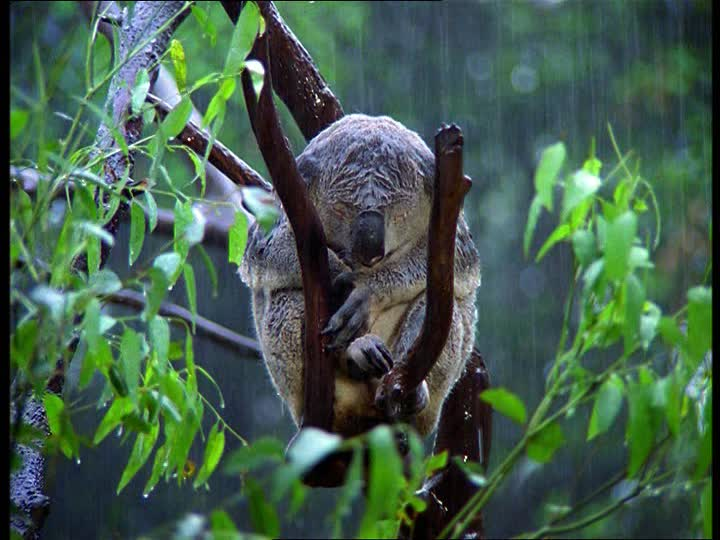
\includegraphics[width=1\textwidth]{koala}
\caption{This is a koala in the rain}
\label{fig:koala}
\end{figure}

To paraphrase Ze Frank, this koala evidences an abundance of apathy regarding its situation.

\subsection{A subsection}

Sometimes it is useful to have two images as part of the same figure.
Figure \ref{fig:unlikelyEvents} shows a cat (briefly) being sweet to a dog and a location that Kramer refers to as the ``nexus of the universe.''

\begin{figure}[ht!]
\centering
\subfloat[]{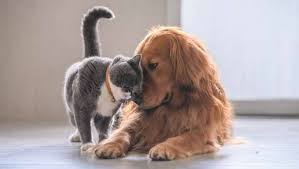
\includegraphics[width=0.45\textwidth]{dogAndCat}}
\subfloat[]{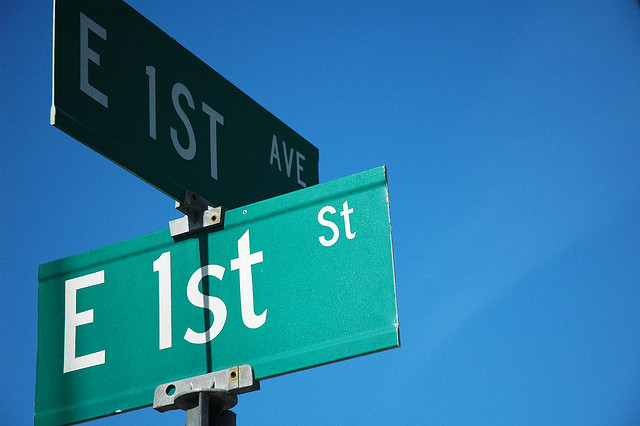
\includegraphics[width=0.45\textwidth]{nexusOfUniverse}}
\caption{Examples of inauspicious events.}
\label{fig:unlikelyEvents}
\end{figure}	

%\input{../Chapters/2perceptionOfDialectVariation.tex}

\input{../Chapters/3variationInIndiana.tex}

\input{../Chapters/4_1_OrientationInIndiana.tex}

\input{../Chapters/4_2_PerceptualDialectMapofIndiana.tex}

\input{../Chapters/5participantsInStatewideStudy.tex}

%\input{../Chapters/6variationInProduction.tex}

\input{../Chapters/7forcedChoice.tex}

\input{../Chapters/8freeClassification.tex}

\input{../Chapters/9conclusion.tex}


\newpage

% \appendix command is necessary to change chapter numbering.
% Appendices are optional

\appendix

\chapter{Word List and Reading Passages}

Below are the word list and reading passages read by the participants in the state-wide study.

\section{Rainbow Passage}

Rainbow Passage (contains a mixture of oral and nasal consonants in the approximate proportion found in everyday speech)
When the sunlight strikes raindrops in the air they act like a prism and form a rainbow. The rainbow is a division of white light into many beautiful colors. These take the shape of a long round arch with its path high above and its two ends apparently beyond the horizon. There is according to legend a boiling pot of gold at one end. When a man looks for something beyond his reach, his friends say he is looking for a pot of gold at the end of the rainbow. 
\vspace{11pt}

\noindent Citation for rainbow passage: Fairbanks, G. (1960). Voice and articulation drillbook, 2nd edn. New York: Harper \& Row. (pp. 124-139).


\section{Mike's Party}

Mike was planning to throw a party on Tuesday night, and decided to check his list one more time before he went shopping. He already had plenty of stuff to drink, and he had enough plates and cups. His brother Jim was going to bring some fish he'd caught and maybe put them on the grill. Mike thought he should get some chips, pretzels, and a few other snacks to start the meal. He looked around to see if he had anything sweet, but then remembered that his friend Linda was baking a cake. When he looked in the cupboard, he saw that he was out of coffee. He found a pencil, wrote it down on his list, and hoped it was on sale. Then he went to the garage, got in his car, and went to the 7-11. It looked like everything would go well.
\vspace{11pt}

\noindent This passage was developed by Dennis Preston and Jon Bakos to target Midland and Southern features


\section{A Bad Day for Ducks}

Tom and Bob were supposed to meet at Tom's house. They planned to got to a nearby pond and watch the ducks. While waiting for Bob to get there, Tom picked up around the house. He put the electric fan away for the winter and did the dishes.

He wanted a snack before he left , so he peeled an apple and cut it into slices. He bit into one, but it was awful, probably rotten. He spit it out and tried to rinse his mouth out with hot black coffee. He poured it into a tin cup, but when he put it up to his lips he spilled it on his hand. His hand puffed up and hurt a lot, so he stuck it under the faucet to make it feel better.

He grabbed a dusty hat out of the closet and shook it, but he couldn't get the dirt off. He got a cap instead and put a scarf around his neck and put on his socks and boots. There was a big hole in his sock, and Bob was really late. It was already past 2:00. Nothing was working out.

Just then Bob phoned and said he wanted to talk. He told Tom that the flock of ducks had left the pond. A pack of dogs had chased them off. Tom was sad; he had really wanted to see the ducks, but Bob said that they could go shoot some pool instead. Tom thought that was a good idea and forgot all about the ducks and his burned hand.

\vspace{11pt}

\noindent This passage was developed by Dennis Preston and students to target Northern Cities features.


\section{Wordlist}

These wordlist items were selected to include key dialect features of the Inland North, Northern, and Southern dialects, especially key features of the Northern Cities Shift, Canadian Raising, Back Vowel fronting, and two phonological mergers as well as vowels in and hVd context.
\vspace{11pt}

\begin{longtable}{lll}
\hline
\textbf{Class} & \textbf{Item} & \textbf{Notes} \\
\hline
\endfirsthead
\multicolumn{3}{c}%
{\textit{Continued from previous page}} \\
\hline
\textbf{Class} & \textbf{Item} & \textbf{Notes} \\
\hline
\endhead
\hline \multicolumn{3}{r}{\textit{Continued on next page}} \\
\endfoot
\hline
\endlastfoot
ae raising       & pal         & sonorant             \\
ae raising       & pan         & sonorant             \\
ae raising       & lag         & velar                \\
ae raising       & pack        & velar                \\
ae raising       & tack        & velar                \\
ae raising       & pat         & alveolar             \\
ae raising       & pad         & alveolar             \\
ae raising       & mad         & alveolar             \\
ae raising       & cap         & labial               \\
wedge            & color       & sonorant             \\
wedge            & lull        & sonorant             \\
wedge            & dull        & sonorant             \\
wedge            & bug         & velar                \\
wedge            & buck        & velar                \\
wedge            & puck        & velar                \\
wedge            & luck        & velar                \\
wedge            & bus         & fricative            \\
wedge            & but         & alveolar             \\
wedge            & cut         & alveolar             \\
wedge            & putt        & alveolar             \\
wedge            & hut         & alveolar             \\
wedge            & cup         & labial               \\
on               & on          & on                   \\
on               & shot        & alveolar             \\
on               & rock        & velar                \\
on               & father      & fricative            \\
on               & got         & alveolar             \\
canadian raising & bike        & ay mono voiceless    \\
canadian raising & cite        & ay mono voiceless    \\
canadian raising & knife       & ay mono voiceless    \\
canadian raising & lice        & ay mono voiceless    \\
canadian raising & life        & ay mono voiceless    \\
canadian raising & pike        & ay mono voiceless    \\
canadian raising & psych       & ay mono voiceless    \\
canadian raising & rice        & ay mono voiceless    \\
canadian raising & write       & ay mono voiceless    \\
canadian raising & writing     & ay bi voiceless      \\
canadian raising & citing      & ay bi voiceless      \\
canadian raising & biting      & ay bi voiceless      \\
canadian raising & buy         & ay mono voiced/pause \\
canadian raising & pie         & ay mono voiced/pause \\
canadian raising & tie         & ay mono voiced/pause \\
canadian raising & ties        & ay mono voiced/pause \\
canadian raising & lies        & ay mono voiced/pause \\
canadian raising & ride        & ay mono voiced/pause \\
canadian raising & rise        & ay mono voiced/pause \\
canadian raising & knives      & ay mono voiced/pause \\
canadian raising & tiger       & ay bi voiced         \\
canadian raising & riding      & ay bi voiced         \\
canadian raising & spider      & ay bi voiced         \\
canadian raising & citation    & ay poly              \\
canadian raising & titanic     & ay poly              \\
canadian raising & psychology  & ay poly              \\
canadian raising & psychotic   & ay poly              \\
canadian raising & gigantic    & ay poly              \\
canadian raising & house       & au                   \\
canadian raising & south       & au                   \\
canadian raising & town        & au                   \\
canadian raising & down        & au                   \\
canadian raising & mouth       & au                   \\
ay monoph        & time        & voiced               \\
ay monoph        & tide        & voiced               \\
ay monoph        & hide        & voiced               \\
ay monoph        & died        & voiced               \\
ay monoph        & tight       & voiceless            \\
ay monoph        & fight       & voiceless            \\
ay monoph        & kite        & voiceless            \\
ay monoph        & might       & voiceless            \\
ay monoph        & bite        & voiceless            \\
u fronting       & dude        &                      \\
u fronting       & food        &                      \\
u fronting       & mood        &                      \\
u fronting       & tube        &                      \\
u fronting       & goose       &                      \\
o fronting       & code        &                      \\
o fronting       & boat        &                      \\
o fronting       & wrote       &                      \\
o fronting       & coat        &                      \\
o fronting       & spoke       &                      \\
o fronting       & goat        &                      \\
low/back         & cot         & a                    \\
low/back         & bot         & a                    \\
low/back         & odd         & a                    \\
low/back         & don         & a                    \\
low/back         & hock        & a                    \\
low/back         & lot         & a                    \\
low/back         & not         & a                    \\
low/back         & stock       & a                    \\
low/back         & caught      & c                    \\
low/back         & bought      & c                    \\
low/back         & awed        & c                    \\
low/back         & dawn        & c                    \\
low/back         & hawk        & c                    \\
low/back         & thought     & c                    \\
low/back         & gnawed      & c                    \\
low/back         & stalk       & c                    \\
pin/pen          & pin         & pin mono             \\
pin/pen          & tin         & pin mono             \\
pin/pen          & bin         & pin mono             \\
pin/pen          & since       & pin mono             \\
pin/pen          & kin         & pin mono             \\
pin/pen          & him         & pin mono             \\
pin/pen          & sinned      & pin mono             \\
pin/pen          & binned      & pin mono             \\
pin/pen          & cinnamon    & pin bi               \\
pin/pen          & ten         & pen mono             \\
pin/pen          & pen         & pen mono             \\
pin/pen          & Ben         & pen mono             \\
pin/pen          & Ken         & pen mono             \\
pin/pen          & hem         & pen mono             \\
pin/pen          & send        & pen mono             \\
pin/pen          & bend        & pen mono             \\
pin/pen          & sense       & pen mono             \\
pin/pen          & pencil      & pen bi               \\
pin/pen          & Tennessee   & pen poly             \\
pin/pen          & sensational & pen poly penultimate \\
hVd              & heed        &                      \\
hVd              & hid         &                      \\
hVd              & hayed       &                      \\
hVd              & head        &                      \\
hVd              & had         &                      \\
hVd              & hod         &                      \\
hVd              & hawed       &                      \\
hVd              & hut         &                      \\
hVd              & hoed        &                      \\
hVd              & hood        &                      \\
hVd              & who’d       &                     
\end{longtable}

\newpage
%\addcontentsline{toc}{chapter}{References}
\bibliographystyle{apacite} % adds the bibliography
\bibliography{dissertationBibliography} % name of .bib file



% Adds a line for your CV without a page number
\newpage

\addtocontents{toc}{%
 \protect\contentsline{chapter}{Curriculum Vitae}{}}

%\begin{center}
%Curriculum Vitae\\
%\textbf{Phillip Weirich}
%\end{center}

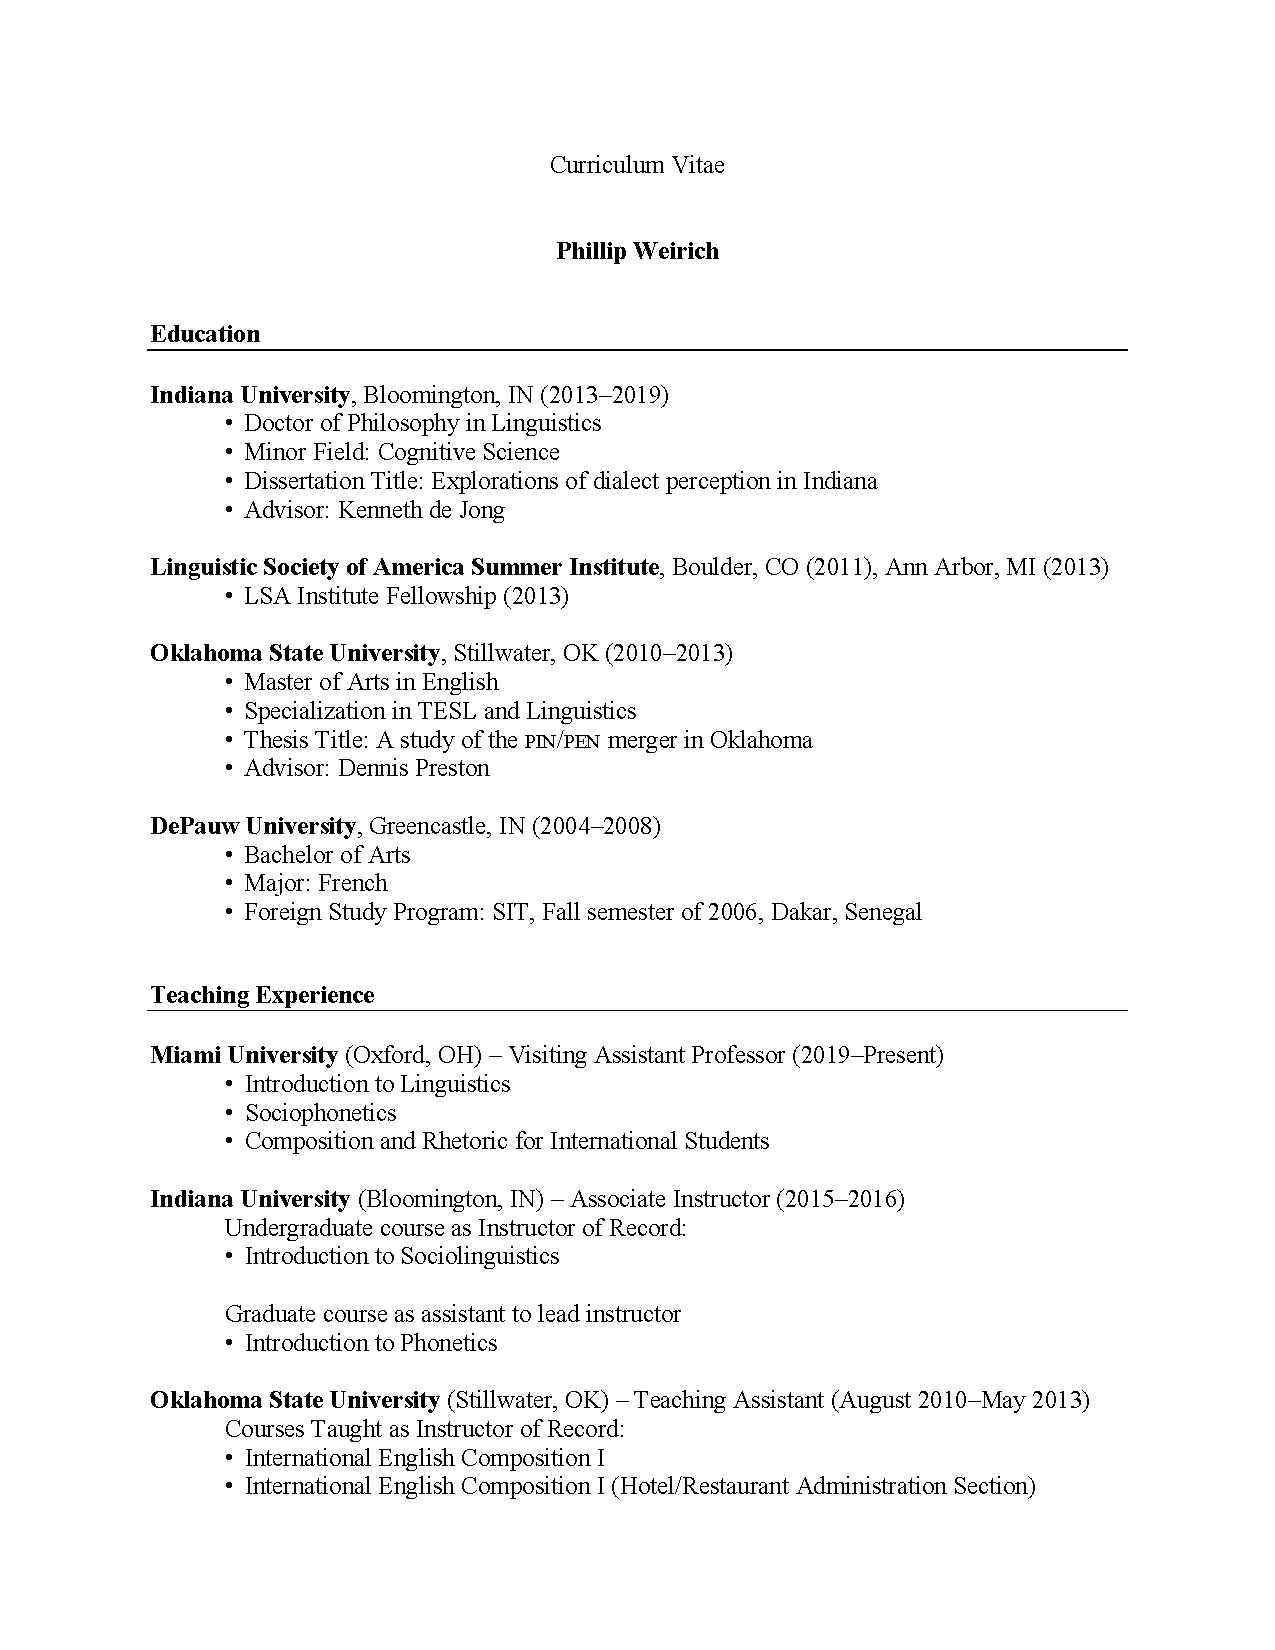
\includepdf[pages=-]{Weirich_CV_28_Sept_2019.pdf} 


\end{document}
